% chktex-file 44
\cleardoublepage
\section{Projekt i Implementacja}

    % ===== ===== ===== =====
    % ANALIZA CELU PRACY
    % ===== ===== ===== ===== 
    \subsection{Analiza celu pracy}
        
        Celem pracy jest stworzenie aplikacji umożliwiającej użytkownikowi zlecanie analiz materiału genetycznego DNA z wielu organizmów, który został pobrany ze środowiska. Aplikacja powinna agregować wyniki tego procesu w formie czytelnej dla człowieka. Będzie ona wykorzystywać bazę danych sekwencji genetycznych. Aplikacja będzie zawierać algorytm grupowania sekwencji oraz wyboru reprezentantów, które zapewnią usprawnienie procesu analiz danych. Zostaną zastosowane modele uczenia maszynowego.

        Najbardziej rozpowszechnioną i stosowaną metodą analizy materiału genetycznego jest klasyfikacja taksonomiczna sekwencji. Pozwala ona określenie, do jakich organizmów nalezą sekwencje zawarte w poddanym analizie materiale genetycznym. Wymaga ona wyszukiwania sekwencji podobnych w bazach danych sekwencji genetycznych do sekwencji analizowanych, a następnie agregację zgromadzonych wyników.

        Wykorzystanie algorytmu grupowania sekwencji genetycznych umożliwi podział sekwencji na grupy sekwencji podobnych, które będą reprezentowane przez wybraną sekwencję zwaną reprezentantem. Wyszukiwanie w bazie danych sekwencji reprezentantów zamiast wszystkich sekwencji znacząco zredukuje liczbę analizowanych sekwencji, co pozwoli na przyśpieszenie całego procesu analizy materiału genetycznego, ponieważ to wyszukiwanie sekwencji podobnych w bazie danych sekwencji jest najbardziej czasochłonnym elementem analizy. Wybór reprezentantów będzie realizowany za pomocą algorytmu, który pozwoli na wybór sekwencji, która najlepiej reprezentuje swoje grupy.

        Ponadto wykorzystanie wysokowydajnego języka programowania pozwoli na minimalizację narzutu obliczeniowego związanego z aplikacją, a zastosowanie ustrukturyzowanego formatu zapisu wyników całego procesu pozwoli na dalsze analizie wyników oraz ich prostą wizualizację.

        Natomiast zastosowanie modeli uczenia maszynowego może usprawnić proces analizy materiału genetycznego oraz zwiększyć jakość wyników otrzymanych za pomocą opisanej optymalizacji poprzez identyfikację ukrytych wzorców i zależności między sekwencjami genetycznymi, które wpływają na ich podobieństwo.


    % ===== ===== ===== =====
    % WYMAGANIA FUNKCJONALNE I NIEFUNKCJONALNE
    % ===== ===== ===== ===== 
    \subsection{Wymagania funkcjonalne i niefunkcjonalne}

        Aby zrealizować postawiony cel, aplikacja musi spełniać wymagania:

        \subsubsection{Wymagania funkcjonalne}

            \begin{itemize}
                \item Aplikacja powinna umożliwiać przeprowadzanie klasyfikacji taksonomicznej dla wprowadzonych sekwencji.
                \item Aplikacja powinna umożliwiać wybór metody grupowania sekwencji genetycznych.
                \item {
                    Aplikacja powinna zawierać zaimplementowane trzy metody grupowania sekwencji genetycznych:
                    \begin{itemize}
                        \item {
                            metodę klasyczną wykorzystującą algorytm Needlemana-Wunscha,
                        }
                        \item {
                            metodę klasyczną wykorzystującą $k$-mery,
                        }
                        \item {
                            nową metodą opartą na sztucznych sieciach neuronowych.
                        }
                    \end{itemize}
                }
                \item Aplikacja powinna umożliwiać porównanie jakości klasyfikacji taksonomicznej wykonanej przy użyciu różnych metod grupowania.
                \item Aplikacja powinna umożliwiać zapis wyników w formacie JSON.
            \end{itemize}

        \subsubsection{Wymagania niefunkcjonalne}

            \begin{itemize}
                \item Aplikacja powinna być wykonana przy wykorzystaniu kompilowanego wysoko wydajnego języka programowania.
                \item Implementacja powinna zawierać testy jednostkowe poszczególnych modułów i funkcji.
            \end{itemize}

    % ===== ===== ===== =====
    % MODEL ARCHITEKTURY C4
    % ===== ===== ===== =====
    \subsection{Model architektury rozwiązania}

        Architektura rozwiązania została przedstawiona w postaci modelu C4\cite{C4}. Model ten opisuje architekturę na czterech poziomach: kontekstowym (ang. \textit{System context}), kontenerów (ang. \textit{Container}), komponentów (ang. \textit{Component}) oraz kodu, przechodząc od najbardziej abstrakcyjnego spojrzenia na architekturę rozwiązania do kodu implementacji. Na rysunku~\ref{Picture:App:C4:Context} przedstawiono diagram kontekstowy modelu architektury, przedstawia on relacje między użytkownikami systemu a systemem oraz relacje między systemem a systemami zewnętrznymi. Na rysunku~\ref{Picture:App:C4:Container} przedstawiono natomiast diagram kontenerów modelu architektury, który przedstawia relacje między użytkownikami a poszczególnymi aplikacjami, biblioteką oraz systemami zewnętrznymi.

        \begin{figure}
            \begin{center}
                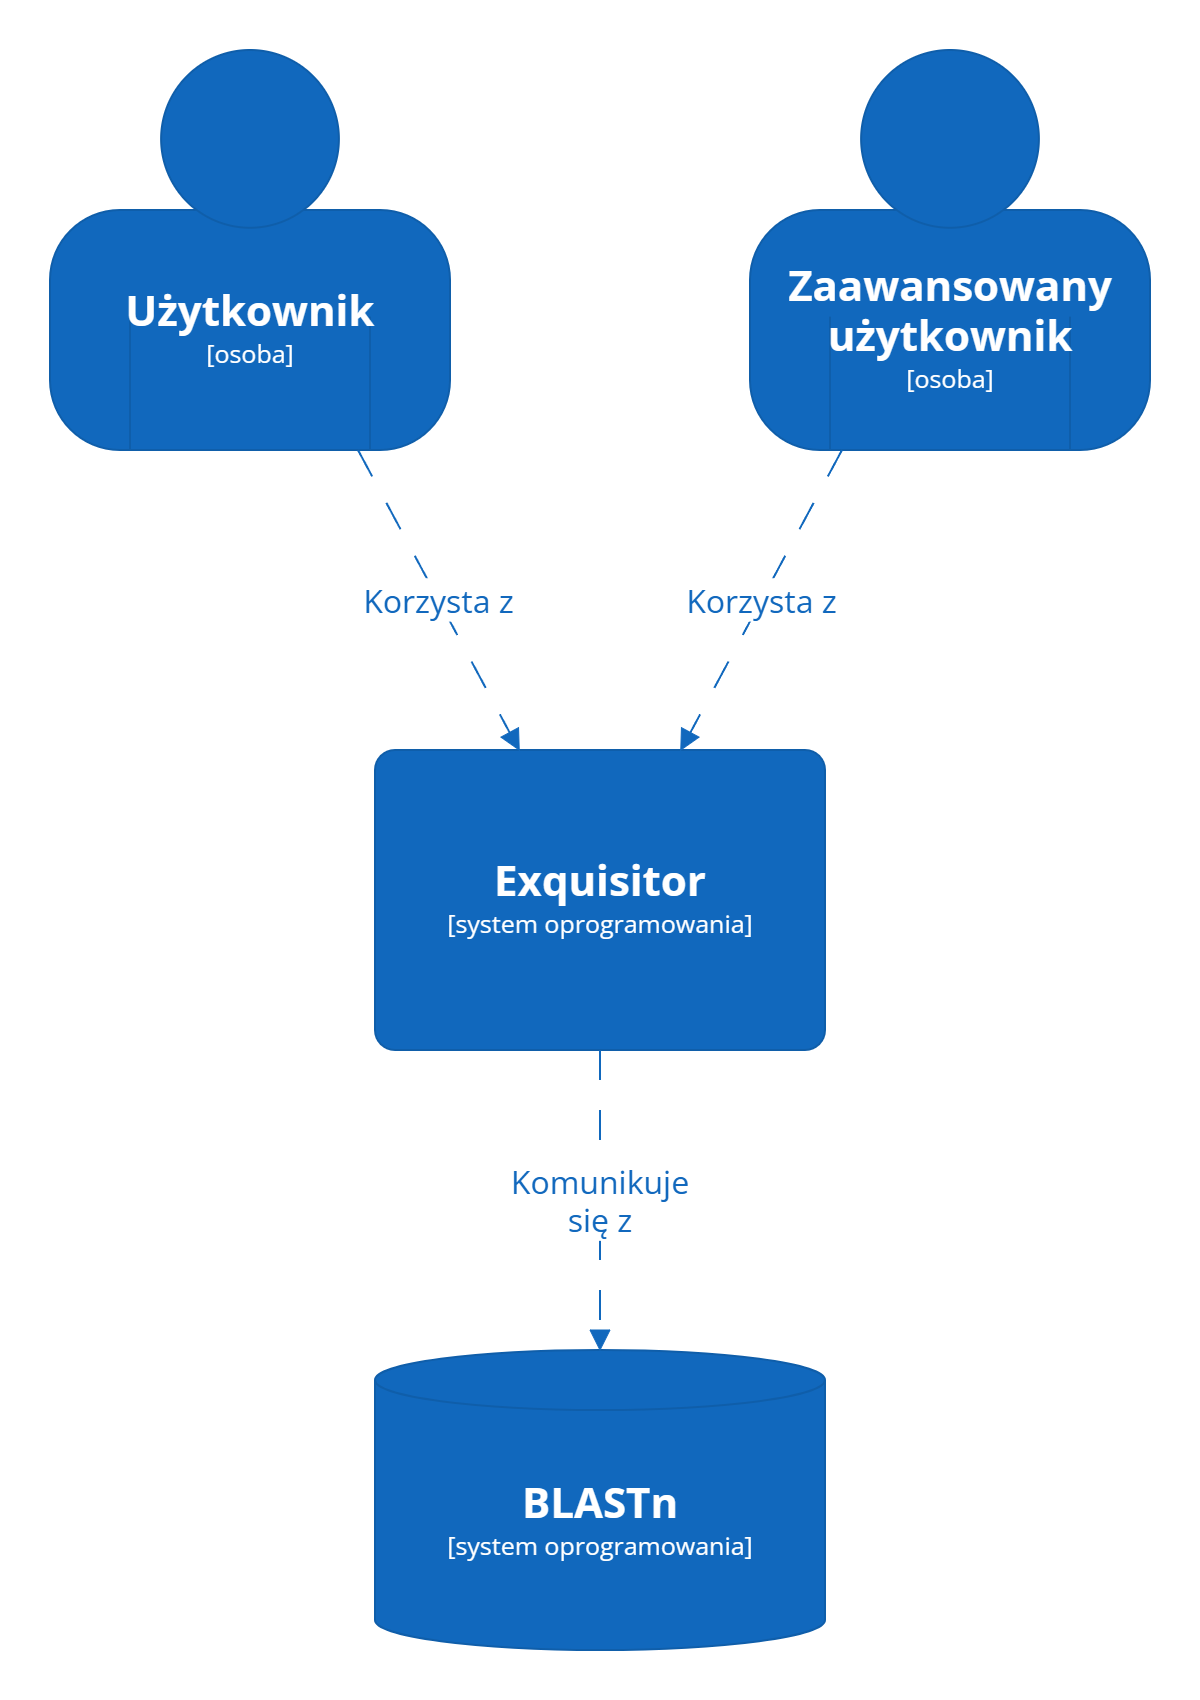
\includegraphics[width=\textwidth]{tex/pictures/app/c4_system_context.png}
            \end{center}
            \caption{
                Diagram kontekstowy modelu architektury.
            }\label{Picture:App:C4:Context}
        \end{figure}

        \begin{figure}
            \begin{center}
                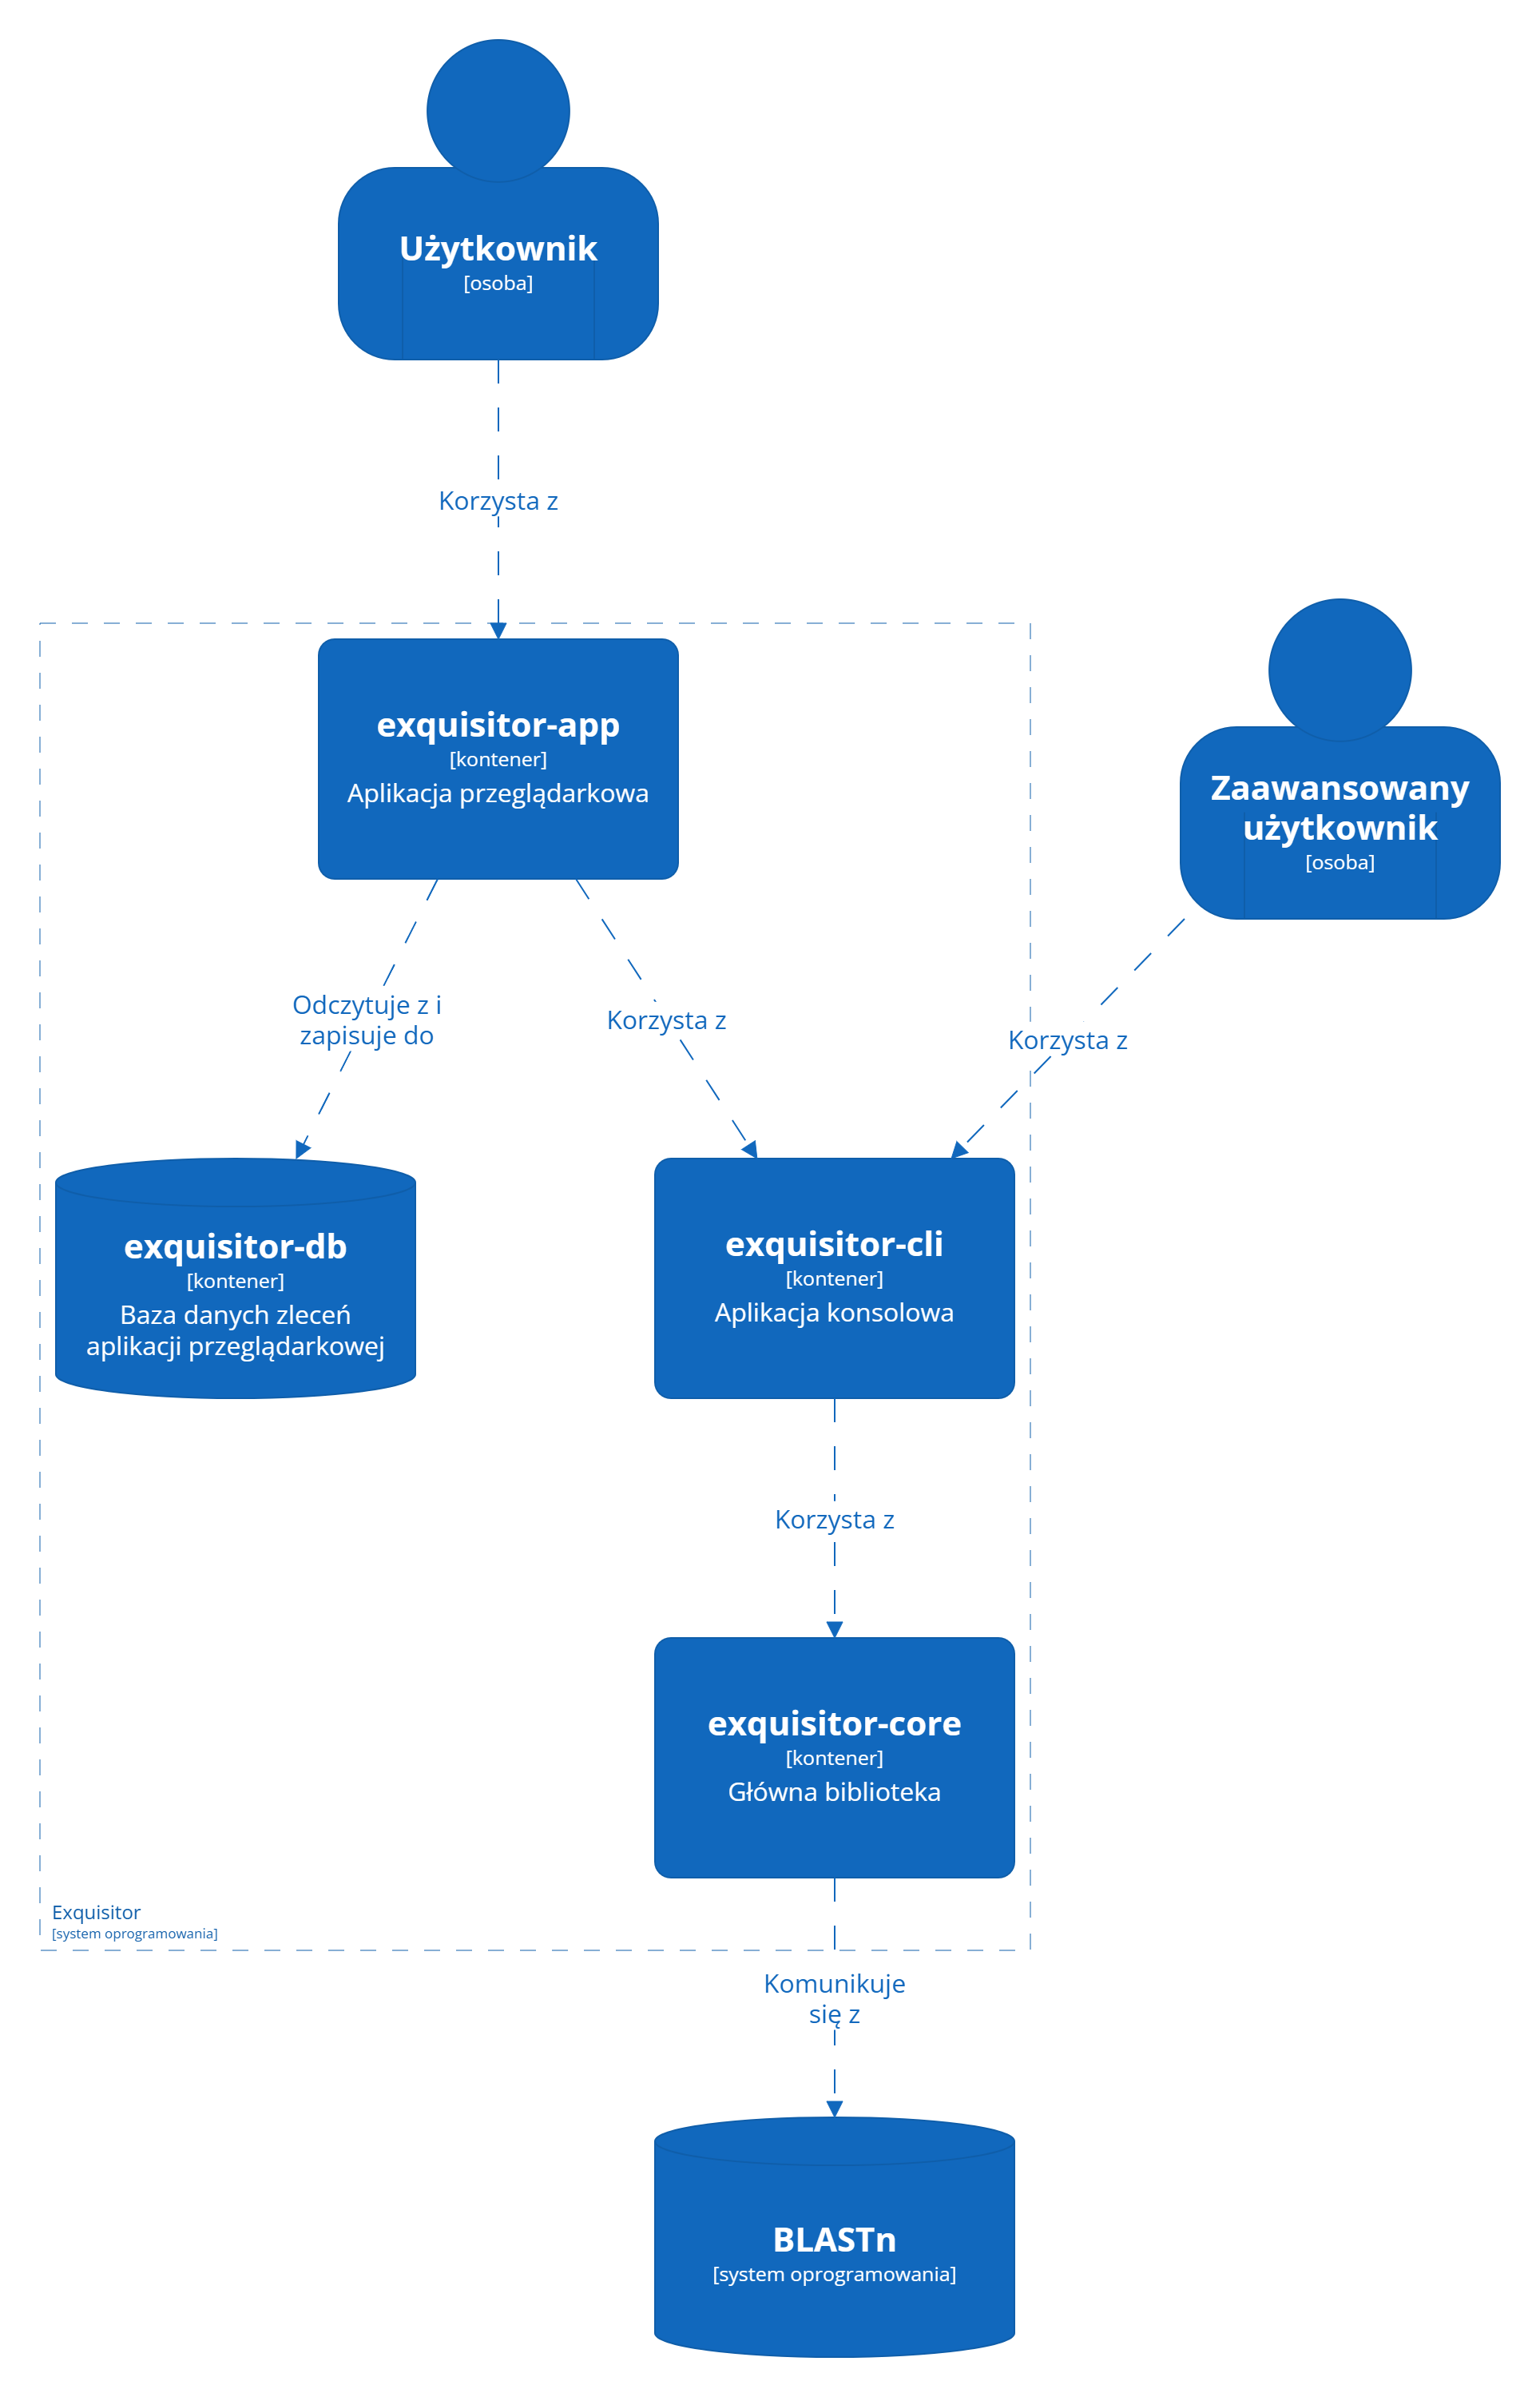
\includegraphics[width=\textwidth]{tex/pictures/app/c4_container.png}
            \end{center}
            \caption{
                Diagram komponentów modelu architektury.
            }\label{Picture:App:C4:Container}
        \end{figure}

    % ===== ===== ===== =====
    % OPIS ROZWIĄZANIA
    % ===== ===== ===== ===== 
    \subsection{Opis rozwiązania}

        Centralnym elementem rozwiązania jest potok przetwarzania, zaprojektowany z myślą o elastycznej konfiguracji oraz możliwości zastosowania różnych metod grupowania sekwencji DNA. Elementy potoku zostały zaimplementowane w bibliotece \textit{exquisitor-core}, w postaci funkcji oraz rekordów. Realizacja potoku została umieszczona w aplikacji konsolowej, która wykorzystuje tę bibliotekę. Aplikacja umożliwia uruchamianie i konfigurację potoku, oferując dostęp do dostępnych metod. Zawiera również polecenia pomocnicze, które zostały przygotowane w celu przeprowadzenia eksperymentów.

        Dodatkowo stworzono aplikację internetową, oferującą prosty interfejs w postaci strony internetowej. Umożliwia ona użytkownikowi zlecanie klasyfikacji taksonomicznej dla przesłanych sekwencji DNA. Do realizacji zleconych zadań aplikacja internetowa korzysta z aplikacji konsolowej.

        Ostatnim komponentem rozwiązania jest sieć neuronowa, której elementy zostały zawarte w bibliotece \textit{exquisitor-core}. 

        Biblioteka, aplikacja konsolowa oraz aplikacja internetowa zostały umieszczone w oddzielnych skrzynkach (ang. \textit{crate}) w ramach jednego rozwiązania. Dzięki temu możliwe jest rozdzielenie odpowiedzialności między poszczególnymi elementami, niezależny rozwój kodu oraz umożliwienie wykorzystania biblioteki w innych aplikacjach.

        % ----- ----- ----- ----- 
        % OPIS POTOKU
        % ----- ----- ----- -----

        \subsubsection{Potok przetwarzania}

            Potok przetwarzania składa się z szeregu kroków, które są realizowane kolejno, jeden po drugim, w celu przeprowadzenia pełnej klasyfikacji taksonomicznej DNA. Każdy krok potoku jest odpowiedzialny za określoną część procesu i może być niezależnie modyfikowany lub wymieniany, co umożliwia elastyczność w doborze metod. Do kluczowych kroków potoku należą:

            \begin{enumerate}
                \item {
                    \textbf{Wstępne przetwarzanie sekwencji}

                    Wejście: \textit{zbiór sekwencji DNA}

                    Wyjście: \textit{zbiór sekwencji DNA}

                    Krok ten odpowiada za weryfikację poprawności dostarczonych sekwencji DNA oraz ich wyrównanie do wymaganej długości, niezbędnej w kolejnych krokach przetwarzania. Może on zostać pominięty, jeśli zastosowana metoda w następnych krokach nie jest wrażliwa na długość sekwencji wejściowych.
                }
                \item {
                    \textbf{Grupowanie sekwencji}

                    Wejście: \textit{zbiór sekwencji DNA}.

                    Wyjście: \textit{Grupy (reprezentant oraz elementy)}.

                    Głównym celem tego kroku jest wybór najlepszych reprezentantów dla każdej grupy sekwencji, która składa się z elementów oraz reprezentanta. Dzięki temu możliwa jest redukcja liczby sekwencji do przetworzenia w kolejnych etapach. Krok ten może zostać zrealizowany przy użyciu jednej z trzech dostępnych metod.
                }
                \item {
                    \textbf{Wyszukiwanie w bazie danych}

                    Wejście: \textit{reprezentanci grup (sekwencje DNA)}.

                    Wyjście: \textit{wykryte organizmy}.

                    Wyszukiwanie w bazie danych sekwencji pozwala znaleźć sekwencje podobne do wyszukiwanych sekwencji DNA. Pozwala to na określenie, do jakich organizmów mogą należeć wyszukiwane sekwencje. W tym kroku przetwarzani są wyłącznie reprezentanci grup. W wyniku wyszukiwania dla każdego reprezentanta uzyskuje się listę odpowiadających organizmów.
                }
                \item {
                    \textbf{Przetwarzanie wyników wyszukiwania}

                    Wejście: \textit{wykryte organizmy, grupy}.

                    Wyjście: \textit{wykryte organizmy}.

                    W tym kroku następuje połączenie informacji o grupach z listą wykrytych organizmów. Obliczane są jakość oraz pewność identyfikacji organizmów na podstawie wyników wyszukiwania uzyskanych w poprzednim kroku oraz liczby elementów w grupach.
                }
                \item {
                    \textbf{Generowanie raportów dla użytkownika}

                    Wyjście: \textit{wykryte organizmy}.

                    Wyjście: \textit{wyniki}.

                    Na podstawie danych z poprzedniego kroku filtrowane są istotne informacje, a następnie generowane są wyniki w formie przystępnej dla użytkownika.
                }
            \end{enumerate}

            Schematyczne przedstawienie potoku zaprezentowano na rysunku~\ref{Picture:Pipeline}. W kółkach umieszczono wejście oraz wyjście z potoku przetwarzania, natomiast w prostokątach – kolejne kroki. Na strzałkach opisano rodzaj przekazywanych danych. Niebieskim kolorem obramowania oznaczono kroki, których wyjściem są sekwencje DNA, czerwonym – kroki, których wyjściem są wykryte organizmy, a zielonym – kroki generujące wyniki w formie czytelnej dla człowieka.

            \begin{figure}
                \begin{center}
                    {
% ===== BEGIN =====
% ----- -----
% COLORS
% ----- -----
\definecolor{Green}{HTML}{1dd1a1}   % Results
\definecolor{Blue}{HTML}{54a0ff}    % Sequences
\definecolor{Yellow}{HTML}{feca57}
\definecolor{Purple}{HTML}{5f27cd}
\definecolor{Grey}{HTML}{576574}
\definecolor{Red}{HTML}{ff6b6b}     % Organisms
\definecolor{Pink}{HTML}{ff9ff3}    
\definecolor{Background}{HTML}{c8d6e5}

% ----- -----
% ELEMENTS
% ----- -----
\tikzstyle{Circle} = [circle, minimum size = 1cm, line width = 2pt, draw=black]
\tikzstyle{Box} = [rectangle, minimum width = 10cm, minimum height = 1.5cm, line width=2pt, text centered, inner sep=10pt, draw=black]
\tikzstyle{Arrow} = [very thick, -Triangle]
\tikzstyle{Arrow:Text} = [pos=0.5, right, font=\footnotesize]

\tikzstyle{seq} = [draw=Blue]
\tikzstyle{db} = [draw=Red]
\tikzstyle{res} = [draw=Green]

% ----- -----
% PICTURE
% ----- -----
\begin{tikzpicture}[node distance=3cm]
    \node (input) [Circle, seq] {Wejście};
    \node (preprocess) [Box, seq, below of=input, align=center] { 1. Wstępne przetwarzanie sekwencji \\ \textbf{(opcjonalnie)} };
    \node (cluster) [Box, seq, below of=preprocess] {2. Grupowanie sekwencji};
    \node (search) [Box, db, below of=cluster] {3. Wyszukiwanie w bazie danych sekwencji};
    \node (postprocess) [Box, db, below of=search] {4. Przetwarzanie wyników wyszukiwania};
    \node (results) [Box, res, below of=postprocess] {5. Generowanie raportów dla użytkownika};
    \node (output) [Circle, res, below of=results] {Wyjście};

    \node (cluster-right) [right of=cluster, xshift=3cm] {};
    \node (postprocess-right) [right of=postprocess, xshift=3cm] { };

    \draw [Arrow, seq] (input) -- (preprocess) node [Arrow:Text] {Zbiór sekwencji DNA};
    \draw [Arrow, seq] (preprocess) -- (cluster) node [Arrow:Text] {Zbiór sekwencji DNA};
    \draw [Arrow, seq] (cluster) -- (search) node [Arrow:Text] {Reprezentaci grup (sekwencje DNA)};
    \draw [Arrow, db] (search) -- (postprocess) node [Arrow:Text] {Wykryte organizmy};
    \draw [Arrow, seq] (cluster.east) -- (cluster-right) -- node [Arrow:Text] {Grupy} (postprocess-right) -- (postprocess.east);
    \draw [Arrow, db] (postprocess) -- (results) node [Arrow:Text] {Wykryte organizmy};
    \draw [Arrow, res] (results) -- (output) node [Arrow:Text] {Wyniki};
\end{tikzpicture}

% ===== END =====
}
                \end{center}
                \caption{
                    Schemat potoku przetwarzania.
                }\label{Picture:Pipeline}
            \end{figure}

        \subsubsection{Biblioteka \textit{exquisitor-core}}
            Podstawę rozwiązania stanowi biblioteka \textit{exqusitor-core} zawarta w skrzynce (ang. \textit{crate}) \textit{exquisitor-core}, stworzona w języku Rust. Zawiera ona implementację wszystkich elementów potoku, które wymagane są przez aplikacje oraz dodatkowo opakowuje implementację algorytmów $k$-medoidów. Biblioteka podzielona jest na kilka modułów ze względu na odpowiedzialność:

            \begin{itemize}
                \item {
                    Moduł \textit{io} odpowiadający za operacje wejścia/wyjścia dla sekwencji DNA zapisanych w formatach FASTA oraz FASTQ. Zawiera on definicje struktur przechowujących sekwencje, metody do ich odczytu i zapisu oraz cechy umożliwiające opis funkcjonalności związanych z obsługą tych formatów.
                }
                \item {
                    Moduł \textit{clustering} realizujący proces grupowania sekwencji DNA na podstawie ich niepodobieństwa. Zawiera metody do obliczania niepodobieństwa między sekwencjami DNA oraz wektorami liczbowymi, a także algorytmy grupowania obiektów. Dodatkowo moduł zawiera strukturę reprezentującą grupę, składającą się z reprezentanta i elementów tej grupy. Zawiera także funkcję do budowy macierzy niepodobieństwa oraz cechy, które definiują interfejs, z którego korzystają inne elementy biblioteki, umożliwia to implementację własnych struktur i funkcji, pozwalając na elastyczne rozszerzanie systemu o nowe metody.
                }
                \item {
                    Moduł \textit{neural}, który zawiera definicję modelu sieci neuronowej, implementację funkcji straty oraz funkcjonalności odpowiedzialnych za wczytanie, oraz przygotowanie danych dla sieci neuronowej, w tym danych uczących. Ponadto zawiera on funkcję trenującą sieć.
                }
                \item {
                    Moduł \textit{searching} zawierający implementację struktur opisujących wykryte organizmy oraz integrację z algorytmem \textit{blastn}.
                }
            \end{itemize}

            W skrzynce \textit{exquisitor-core} znajdują się dwa dodatkowe programy – pierwszy służy do przygotowania danych uczących dla sieci neuronowej i eksperymentalnych poprzez losowanie próbek z większego zbioru danych, natomiast drugi odpowiada za uczenie sieci neuronowej.

        \subsubsection{Aplikacja konsolowa \textit{exquisitor-cli}}
            Główną aplikacją, która implementuje pełny potok przetwarzania i realizuje klasyfikację taksonomiczną, jest aplikacja konsolowa \textit{exquisitor-cli} zawarta w skrzynce o tej samej nazwie. Aplikacja oferuje standardowy interfejs użytkownika typowy dla aplikacji konsolowych i wykonuje komendy wywołane przez użytkownika. Interfejs tekstowy umożliwia uruchamianie aplikacji w środowiskach bez dostępu do środowiska graficznego.

            Aplikacja implementuje następujące komendy:
            \begin{itemize}
                \item {
                    \textit{experiment} --- umożliwia uruchomienie wskazanej komendy w ramach eksperymentu. Pozwala na monitorowanie wykorzystania pamięci RAM oraz procesora, oraz określenie maksymalnego czasu trwania eksperymentu, po których zostanie przerwany. Wykorzystywana jest do przeprowadzania eksperymentów. W wyniku działania generuje plik w formacie CSV zawierający monitorowane dane z zadaną rozdzielczością.
                }
                \item {
                    \textit{compare} --- pozwala na porównanie dwóch zestawów wyników klasyfikacji taksonomicznej, wyliczając jakość względną jednego zestawu do drugiego. Wyniki są wyświetlane na ekranie lub, w przypadku podania ścieżki, zapisywane do pliku.
                }
                \item {
                    \textit{compare-clusters} --- pozwala na porównanie jakości dwóch zestawów grup, które zostały otrzymane w wyniku zastosowania algorytmu grupowania.
                }
                \item {
                    \textit{search} --- pozwala na wyszukanie sekwencji w bazie danych bez wykonywania całego potoku przetwarzania. Wyniki działania komendy zapisywane są we wskazanym pliku.
                }
                \item {
                    \textit{run} --- jest główną komendą, która realizuje potok przetwarzania. Uruchamia potok przetwarzania dla sekwencji DNA zawartych w podanym pliku. Pozwala na konfigurację wykorzystywanej metody grupowania sekwencji, algorytmu grupowania sekwencji oraz ich parametrów. Dodatkowo umożliwia zapisanie grup otrzymanych w wyniku grupowania. Wymaga podania ścieżki do programu \textit{blastn} oraz ścieżki do jego bazy danych. Wyniki zapisuje do pliku, a w przypadku braku podania ścieżki na ekranie.
                }
            \end{itemize}

        \subsubsection{Aplikacja internetowa \texttt{exquisitor-app}}
            Aplikacja internetowa została zaprojektowana z myślą o umożliwieniu użytkownikom końcowym zlecania zadań klasyfikacji taksonomicznej oraz przeglądania wyników po zakończeniu procesu. Wybór formy aplikacji internetowej wynika z jej dostępności na różnych urządzeniach posiadających dostęp do internetu i przeglądarki, co zapewnia łatwy, uniwersalny dostęp do systemu. Aplikacja składa się z serwera oraz stron internetowych generowanych za pomocą szablonów.

            Serwer udostępnia stronę główną, na której użytkownik może zapoznać się z ostatnimi dziesięcioma zadaniami, zlecić wykonanie nowego zadania lub wyszukać zadanie po identyfikatorze, lub nazwie. Do przechowywania informacji o zleconych zadaniach wykorzystywana jest baza danych \textit{SQLite}.
            
            Do głównych funkcji serwera należą:
            \begin{itemize}
                \item Generowanie stron internetowych na podstawie szablonów.
                \item Serwowanie statycznych plików CSS oraz JavaScript.
                \item Obsługa błędów i wyświetlanie stosownych komunikatów dla użytkownika.
            \end{itemize}
            
            Schemat bazy danych znajduje się na rysunku~\ref{Picture:App:Database}.

            \begin{figure}
                \begin{center}
                    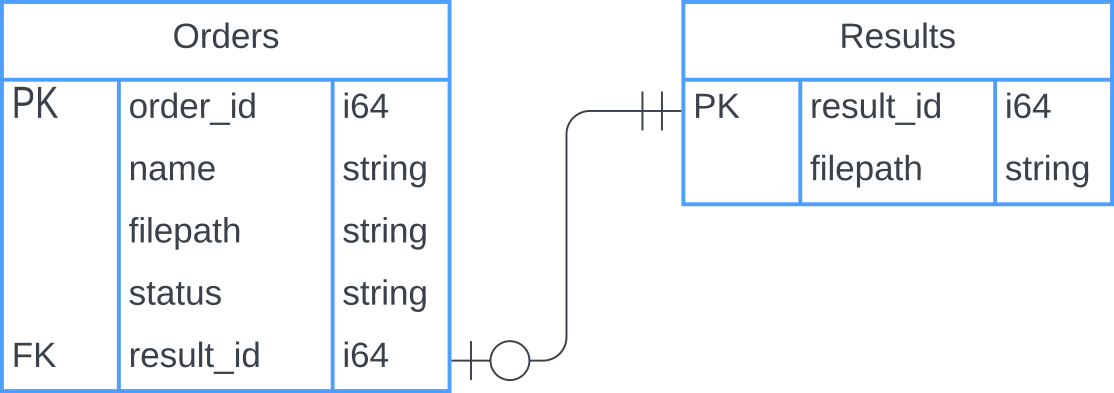
\includegraphics[width=\textwidth]{tex/pictures/app/database.png}
                \end{center}
                \caption{
                    Diagram ER modelu bazy danych aplikacji internetowej.
                }\label{Picture:App:Database}
            \end{figure}

    % ===== ===== ===== =====
    % METODY
    % ===== ===== ===== =====
    \subsection{Metody grupowania sekwencji}

        W pracy zaimplementowano trzy metody grupowania sekwencji DNA. Każda metoda składa się z wyznaczania niepodobieństwa między sekwencjami DNA, które służą do budowy macierzy niepodobieństwa, a następnie do przeprowadzenia grupowania sekwencji. Każda z metod obejmuje:

        \begin{itemize}
            \item {wyznaczenie niepodobieństwa między sekwencjami,}
            \item {budowę macierzy niepodobieństwa,}
            \item {zastosowanie algorytmu grupowania.}
        \end{itemize}

        Budowanie macierzy niepodobieństwa oraz zastosowanie algorytmu grupowania wygląda we wszystkich metodach jednakowo. W dalszych sekcjach opisany zostanie proces wyznaczania niepodobieństwa między sekwencjami w zaimplementowanych metodach.
        
        \subsubsection{Zmodyfikowany algorytm Needlemana-Wunscha}\label{Method:NeedlemanWunsch}

            Pierwszą metodą zastosowaną do wyznaczenia niepodobieństwa między sekwencjami DNA jest  zmodyfikowany algorytm Needlamana-Wunscha. Algorytm ten pierwotnie służy do globalnego wyrównania sekwencji genetycznych. Korzystając z własności algorytmu, że w komórce $D_{n+1, m+1}$ macierzy podobieństwa budowanej przez algorytm znajduje się jakość globalnego wyrównania, dokonano modyfikacji algorytmu oraz odpowiedniego ustawienia parametrów, aby wynik ten odpowiadał mierze niepodobieństwa między sekwencjami. Modyfikacje te polegały na zmianie budowy macierzy podobieństwa oraz wprowadzeniu dodatkowych ograniczeń, w celu zapewnienia, że wartość w $D_{n+1, m+1}$ będzie zawierała się w przedziale $[0, \infty)$. Szczegóły wprowadzonych zmian względem wyrażenia \eqref{Equation:NeedlemanWunsch} przedstawiono poniżej:

            \begin{equation}
                \begin{aligned}
                    D_{i,j} &= \min
                    \begin{cases}
                    D_{i - 1, j} + g \\
                    D_{i, j - 1} + g \\
                    D_{i - 1, j - 1} + s(A_{i - 1}, B_{j - 1})
                    \end{cases}, & \text{dla } & i \in \left(1, n + 1\right] \text{ oraz } j \in \left(1, m + 1\right] \\
                    & g, s(A_i, B_j) \in \mathbb{R}^{+}
                \end{aligned}
            \end{equation}

            gdzie,
            \begin{align*} 
                A, B -& \text{porównywane sekwencje}, \\
                n, m -& \text{długości sekwencji } A \text{ oraz } B, \\
                D -& \text{macierz podobieństwa o rozmiarach } (n + 1) \text{ x } (m + 1), \\
                g -& \text{kara za przerwę}, \\
                s(A_i, B_j) -& \text{podobieństwo między  } i\text{-tym elementem w sekwencji A,} \\ 
                & \text{a } j \text{-tym elementem w sekwencji B}. \\
            \end{align*}

            W rozwiązaniu przyjęto wartości parametrów:
            \begin{align*}
                g &= 2, \\
                s(a, b) &= \begin{cases}
                    0, & \text{dla } a = b, \\
                    1, & \text{dla } a \neq b.
                \end{cases}
            \end{align*}

            Pełny przebieg metody przedstawiono na schemacie~\ref{Picture:Cluster:NeedlemanWunsch}. Czerwonym obramowaniem oznaczono krok, w którym wykorzystywany jest zmodyfikowany algorytm Needlemana-Wunscha.

            \paragraph{Przykład.} Macierz podobieństwa zbudowana dla sekwencji \texttt{ACT} oraz \texttt{GCA} przy użyciu zmodyfikowanego algorytmu Needlemana-Wunscha, z uwzględnieniem przyjętych parametrów będzie wyglądać następująco:

            \[
                \begin{matrix}
                            &        & A      & C      & T      \\
                            &      0 &      2 &      4 &      6 \\
                     G      &      2 &      1 &      3 &      5 \\
                     C      &      4 &      3 &      1 &      3 \\
                     A      &      6 &      4 &      3 &      2 \\
                \end{matrix}
            \]

            Niepodobieństwo między tymi sekwencjami, zawarte w komórce $D_{n + 1, m + 1}$ wynosi zatem $2$.

            \begin{figure}
                \begin{center}
                    {
% ===== BEGIN =====
% ----- -----
% COLORS
% ----- -----
\definecolor{Green}{HTML}{1dd1a1}
\definecolor{Blue}{HTML}{54a0ff}
\definecolor{Yellow}{HTML}{feca57}
\definecolor{Purple}{HTML}{5f27cd}
\definecolor{Grey}{HTML}{576574}
\definecolor{Red}{HTML}{ff6b6b}
\definecolor{Pink}{HTML}{ff9ff3}
\definecolor{Background}{HTML}{c8d6e5}

% ----- -----
% ELEMENTS
% ----- -----
\tikzstyle{Circle} = [circle, minimum size=1cm, line width=2pt, draw=black]
\tikzstyle{Box} = [rectangle, minimum width=10cm, minimum height=1.5cm, line width=2pt, text centered, inner sep=10pt, draw=black]
\tikzstyle{Arrow} = [very thick, -Triangle]
\tikzstyle{Arrow:Text} = [pos=0.5, right, font=\footnotesize]

% ----- -----
% PICTURE
% ----- -----
\begin{tikzpicture}[node distance=3cm]
    \node (input) [Circle] { Wejście };
    \node (distance) [Box, below of=input, align=center, draw=Red] { 1. Obliczenie niepodobieństwa między sekwencjami \\ \textbf{za pomocą algorytmu Needlemana-Wunscha} };
    \node (matrix) [Box, below of=distance] { 2. Stworzenie macierzy niepodoobieństwa };
    \node (cluster) [Box, below of=matrix, align=center] { 3. Grupowanie sekwencji \\ \textbf{za pomocą algorytmu k-medoidów}};
    \node (output) [Circle, below of=cluster] { Wyjście };

    \draw [Arrow] (input) -- (distance) node [Arrow:Text] {Zbiór sekwencji DNA};
    \draw [Arrow] (distance) -- (matrix) node [Arrow:Text] {Niepodobieństwo sekwencji};
    \draw [Arrow] (matrix) -- (cluster) node [Arrow:Text] {Macierz niepodobieństwa};
    \draw [Arrow] (cluster) -- (output) node [Arrow:Text] {Grupy};
\end{tikzpicture}

% ===== END =====
}
                \end{center}
                \caption{
                    Grupowanie sekwencji z wykorzystaniem zmodyfikowanego algorytmu Needlemana-Wunscha do określenia niepodobieństwa między sekwencjami.
                }\label{Picture:Cluster:NeedlemanWunsch}
            \end{figure}

        \subsubsection{Metoda zanurzeń \textit{k-merów}}
            Metoda zanurzeń \textit{k-merów} jest drugą klasyczną metodą wyznaczania niepodobieństwa między sekwencjami genetycznymi, w tym sekwencjami DNA. Polega ona na wyznaczeniu wszystkich \textit{k-merów} dla sekwencji wejściowych, a następnie obliczeniu niepodobieństwa sekwencji poprzez porównanie liczby wystąpień danych \textit{k-merów} w porównywanych sekwencjach.

            Z wyznaczonych \textit{k-merów} tworzy się wektor zanurzeń, w którym każda pozycja odpowiada określonemu \textit{k-merowi}. Przykładowo, dla \textit{k} = 2 (k-mery dwuznakowe) możemy przypisać odpowiednią pozycję w wektorze do każdego możliwego k-meru, np.:
            
            \[
            \text{AA} \to 0, \quad \text{AC} \to 1, \quad \text{AT} \to 2, \quad \text{AG} \to 3, \quad \text{CA} \to 4, \quad \dots
            \]
            
            Wektor zanurzeń dla danej sekwencji DNA zawiera liczbę wystąpień każdego \textit{k-meru} w odpowiednich pozycjach. Na przykład, dla sekwencji `AAACA' wektor zanurzeń dla $k=2$ może wyglądać następująco:
            
            \[
            \text{AAACA} \to [2, 1, 0, 0, 1, \dots]
            \]
            
            gdzie liczba na pozycji 0 oznacza liczbę wystąpień \textit{AA} w sekwencji, liczba na pozycji 1 oznacza liczbę wystąpień \textit{AC}, itd. Następnie, na podstawie tych wektorów zanurzeń, oblicza się niepodobieństwo między sekwencjami, porównując ich wektory zanurzeń według wzoru:

            \begin{equation}
                dissimilarity_{kmer}(A, B, k) = \sqrt{\sum_{m \in M_{k}} (A_m - B_m)^{2}}
            \end{equation}

            gdzie,
            \begin{align*} 
                k -& \text{długość $k$-merów}, \\
                A, B -& \text{porównywane sekwencje}, \\
                M -& \text{zbiór wszystkich możliwych sekwencji genetycznych o długości $k$}, \\
                A_j, B_j -& \text{liczba wystąpień sekwencji } j \text{ odpowiednio w sekwencjach } A \text{ i } B. \\
            \end{align*}

            Pełny przebieg wykorzystania metody zanurzeń \textit{k-merów} w grupowaniu sekwencji został pokazany na schemacie~\ref{Picture:Cluster:KMer}. Czerwonym obramowaniem oznaczono krok, w którym wykorzystana została metoda.

            \begin{figure}
                \begin{center}
                    {
% ===== BEGIN =====
% ----- -----
% COLORS
% ----- -----
\definecolor{Green}{HTML}{1dd1a1}
\definecolor{Blue}{HTML}{54a0ff}
\definecolor{Yellow}{HTML}{feca57}
\definecolor{Purple}{HTML}{5f27cd}
\definecolor{Grey}{HTML}{576574}
\definecolor{Red}{HTML}{ff6b6b}
\definecolor{Pink}{HTML}{ff9ff3}
\definecolor{Background}{HTML}{c8d6e5}

% ----- -----
% ELEMENTS
% ----- -----
\tikzstyle{Circle} = [circle, minimum size=1cm, line width=2pt, draw=black]
\tikzstyle{Box} = [rectangle, minimum width=10cm, minimum height=1.5cm, line width=2pt, text centered, inner sep=10pt, draw=black]
\tikzstyle{Arrow} = [very thick, -Triangle]
\tikzstyle{Arrow:Text} = [pos=0.5, right, font=\footnotesize]

% ----- -----
% PICTURE
% ----- -----
\begin{tikzpicture}[node distance=3cm]
    \node (input) [Circle] { Wejście };
    \node (embed) [Box, below of=input, draw=Red] { 1. Stworzenie zanurzeń k-merów };
    \node (distance) [Box, below of=embed, align=center] { 2. Obliczenie niepodobieństwa \\ między wektorami zanurzeń };
    \node (matrix) [Box, below of=distance] { 3. Stworzenie macierzy niepodoobieństwa };
    \node (cluster) [Box, below of=matrix, align=center] { 4. Grupowanie sekwencji \\ \textbf{za pomocą algorytmu k-medoidów}};
    \node (output) [Circle, below of=cluster] { Wyjście };

    \draw [Arrow] (input) -- (embed) node [Arrow:Text] {Zbiór sekwencji DNA};
    \draw [Arrow] (embed) -- (distance) node [Arrow:Text] {Wektory zanurzeń};
    \draw [Arrow] (distance) -- (matrix) node [Arrow:Text] {Niepodobieństwo sekwencji};
    \draw [Arrow] (matrix) -- (cluster) node [Arrow:Text] {Macierz niepodobieństwa};
    \draw [Arrow] (cluster) -- (output) node [Arrow:Text] {Grupy};
\end{tikzpicture}

% ===== END =====
}
                \end{center}
                \caption{
                    Grupowanie sekwencji z wykorzystaniem zanurzeń \textit{k-merów} do określenia niepodobieństwa między sekwencjami.
                }\label{Picture:Cluster:KMer}
            \end{figure}

        \subsubsection{Sztuczna sieć neuronowa}

            Nową zaproponowaną metodą jest wykorzystanie sztucznej sieci neuronowej do redukcji wymiarowości wejściowych sekwencji DNA do postaci wektora cech o wymiarze $\mathbb{R}^{64}$. Sztuczna sieć neuronowa wykorzystuje uczenie kontrastowe, które umożliwia naukę reprezentacji danych wejściowych z zachowaniem własności podobieństwa oraz niepodobieństwa między wejściowymi sekwencjami. Niepodobieństwo między sekwencjami zostanie obliczone poprzez obliczenie niepodobieństwa kosinusowego wyrażonego wzorem~\eqref{Equation:CosineDissimilarity} między wektorami cech sekwencji DNA.

            \paragraph{Architektura}
                Architektura modelu sztucznej sieci neuronowej składa się z dwóch bloków splotowych oraz bloku perceptronów wielowarstwowych. Każdy z bloków splotowych zawiera warstwę splotową oraz warstwę normalizacji wsadowej i jest odpowiedzialny za ekstrakcję niskopoziomowych cech sekwencji. Ostatni blok splotowy jest połączony z blokiem perceptronów wielowarstwowych za pomocą warstwy spłaszczającej. Blok perceptronów wielowarstwowych odpowiada za tworzenie reprezentacji sekwencji, składa się z trzech warstw, które wykorzystują funkcję aktywacji GELU\cite{Hendrycks:2016}, z wyjątkiem ostatniej warstwy. Wyjściem całego modelu jest wektor cech o wymiarze $\mathbb{R}^{64}$.

                Schematycznie architektura została przedstawiona na rysunku~\ref{Picture:NeuralModel}. 

                \begin{figure}
                    \begin{center}
                        {
% ===== BEGIN =====
% ----- -----
% COLORS
% ----- -----
\definecolor{Green}{HTML}{1dd1a1}   % Input
\definecolor{Blue}{HTML}{54a0ff}    % Linear
\definecolor{Yellow}{HTML}{feca57}  % Convolution
\definecolor{Purple}{HTML}{5f27cd}  % Batch Norm
\definecolor{Grey}{HTML}{576574}    % Dropout
\definecolor{Red}{HTML}{ff6b6b}     % Output
\definecolor{Pink}{HTML}{ff9ff3}    % Activation
\definecolor{Background}{HTML}{c8d6e5}

% ----- -----
% ELEMENTS
% ----- -----
\tikzstyle{box} = [rectangle, rounded corners, minimum width=5cm, minimum height=1cm, text centered, draw=black, align=center]
\tikzstyle{input} = [box, fill=Green!30]
\tikzstyle{linear} = [box, fill=Blue!30]
\tikzstyle{conv} = [box, fill=Yellow!30]
\tikzstyle{bn} = [box, fill=Purple!30]
\tikzstyle{activation} = [box, fill=Pink!30]
\tikzstyle{dropout} = [box, fill=Grey!30]
\tikzstyle{output} = [box, fill=Red!30]

\tikzstyle{arrow} = [very thick, -Triangle]
\tikzstyle{arrow:text} = [pos=0.5, right, font=\footnotesize]

% ----- -----
% PICTURE
% ----- -----
\begin{tikzpicture}[node distance=2cm]
    \node (input) [input] { Wejście };
    \node (conv1) [conv, below of=input] { Splot 1D \\ \textbf{16@1x16, krok: 4} };
    \node (bn1) [bn, below of=conv1] { Normalizacja wsadowa };
    \node (conv2) [conv, below of=bn1] { Splot 1D \\ \textbf{32@1x8} };
    \node (bn2) [bn, below of=conv2] { Normalizacja wsadowa };
    \node (flatten) [linear, below of=bn2] { Warstwa spłaszczająca };
    \node (flatten-right) [right of=flatten, xshift=2cm] {};
    
    \node (fc1-left) [right of=input, xshift=2cm] {};
    \node (fc1) [linear, right of=input, xshift=6cm] { Warstwa gęsta };
    \node (act1) [activation, below of=fc1] { Aktywacja \\ \textbf{GELU} };
    \node (drop1) [dropout, below of=act1] { Wyłączenie neuronów };
    \node (fc2) [linear, below of=drop1] { Warstwa gęsta };
    \node (act2) [activation, below of=fc2] { Aktywacja \\ \textbf{GELU} };
    \node (drop2) [dropout, below of=act2] { Wyłączenie neuronów };
    \node (fc3) [linear, below of=drop2] { Warstwa gęsta };
    \node (output) [output, below of=fc3] { Wyjście };

    \draw [arrow] (input) -- (conv1) node [arrow:text] {1x600};
    \draw [arrow] (conv1) -- (bn1) node [arrow:text] {16x147};
    \draw [arrow] (bn1) -- (conv2) node [arrow:text] {16x147};
    \draw [arrow] (conv2) -- (bn2) node [arrow:text] {32x140};
    \draw [arrow] (bn2) -- (flatten) node [arrow:text] {32x140};

    \draw [arrow] (flatten.east) -- (flatten-right) -- node [arrow:text] {1x4480} (fc1-left) -- (fc1.west);
    \draw [arrow] (fc1) -- (act1) node [arrow:text] {1x4096};
    \draw [arrow] (act1) -- (drop1) node [arrow:text] {1x4096};
    \draw [arrow] (drop1) -- (fc2) node [arrow:text] {1x4096};
    \draw [arrow] (fc2) -- (act2) node [arrow:text] {1x512};
    \draw [arrow] (act2) -- (drop2) node [arrow:text] {1x512};
    \draw [arrow] (drop2) -- (fc3) node [arrow:text] {1x512};
    \draw [arrow] (fc3) -- (output) node [arrow:text] {1x64};
\end{tikzpicture}

% ===== END =====
}
                    \end{center}
                    \caption{
                        Schemat architektury sieci neuronowej.
                    }\label{Picture:NeuralModel}
                \end{figure}

            \paragraph{Dane wejściowe}
                Wejściem modelu są sekwencje DNA o długości $150$, które są zakodowane do postaci wektora o wymiarach $1x600$ za pomocą kodu 1 z n\cite{HarrisDavid:2007}.
            
            \paragraph{Przykłady uczące}
                Przykłady uczące oraz walidacyjne składają się z kotwicy (ang. \textit{anchor}), sekwencji pozytywnej (ang. \textit{positive}), czyli podobnej do kotwicy oraz sekwencji negatywnej (ang. \textit{negative}) niepodobnej do kotwicy.
            
            \paragraph{Zbiór danych}
                Zbiór danych uczących oraz walidacyjnych został stworzony na podstawie pierwszej próbki sekwencji genetycznych ze zbioru \textit{CAMI II Toy Human Microbiome Project}\cite{Fritz:2019}. Próbka zawiera symulowane dane metagenomiczne z mikrobiomu skóry człowieka. Przykłady zostały uzyskane poprzez losowanie kotwic ze zbioru oraz modyfikację tych kotwic w celu stworzenia sekwencji pozytywnej i negatywnej. Modyfikacja polegała na zamianie punktowej danego nukleotydu na inny. W przypadku sekwencji pozytywnej zmiana obejmowała od $0\%$ do $20\%$ długości kotwicy, natomiast w przypadku sekwencji negatywnej od $20\%$ do $80\%$ długości kotwicy.

            \paragraph{Funkcja straty}
                Wykorzystano funkcję straty zdefiniowaną jako:

                \begin{equation}
                    \text{Strata kontrastowa} = [m_{pos} - s_{pos}]_{+} + [s_{neg} - m_{neg}]_{+}
                \end{equation}

                gdzie,
                \begin{align*}
                    m_{pos} &- \text{margines podobieństwa między sekwencją pozytywną a kotwicą,} \\
                    m_{neg} &- \text{margines podobieństwa między sekwencją negatywną a kotwicą,} \\
                    s_{pos} &- \text{podobieństwo kosinusowe sekwencji pozytywnej do kotwic,} \\
                    s_{pos} &- \text{podobieństwo kosinusowe sekwencji negatywnej do kotwic.} \\
                \end{align*}

            \paragraph{Proces uczenia}
                Proces uczenia modelu sieci neuronowej został przeprowadzony na zbiorze $10^{6}$ przykładów uczących oraz $10^{4}$ przykładów walidacyjnych. 
                W procesie wykorzystano optymalizator \textit{AdamW}\cite{Loshchilov2017DecoupledWD} z wykładniczym spadkiem współczynnika uczenia oraz zanikiem wag (ang. \textit{weight decay}).
            
            \paragraph{Miara jakości}
                Jako miarę jakości modelu wykorzystano stratę kontrastową modelu obliczoną na zbiorze walidacyjnym.

            \paragraph{Parametry procesu uczenia}
                Przeprowadzono eksperymenty w celu określenia optymalnych parametrów uczenia modelu sztucznej sieci neuronowej. Sprawdzono parametry współczynnika uczenia $\lambda$, zaniku wag $w$, współczynnika $\gamma$ stosowanego w wykładniczym spadku współczynnika uczenia, parametr wyłączania neuronów oraz stosowność trzech warstw perceptronów. W wyniku eksperymentów wybrano najlepsze parametry: $\lambda = 10^{-6}$, $w = $, $\gamma=0.99999$, współczynnik wyłączenia neuronów na poziomie $0.5$ oraz stwierdzono pozytywny wpływ zastosowania trzech warstw perceptronów. 
                Wykorzystano również funkcję straty z parametrami: $m_{pos} = 1.0$, $m_{neg} = 0.25$.

            \paragraph{Wyniki procesu uczenia}
                
                W wyniku procesu uczenia modelu sztucznej sieci neuronowej, po 3 epokach uzyskano model, który osiągnął stratę równą $0.117$ na zbiorze walidacyjnym. Liczba epok została wybrana na podstawie analizy procesu uczenia, w którym po tej liczbie epok zaobserwowano nadmierne dopasowywanie się modelu (ang. \textit{overfitting}).


            Pełne wykorzystanie sztucznej sieci neuronowej w grupowaniu sekwencji zostało przedstawione na rysunku~\ref{Picture:Cluster:Neural}. Czerwonym obramowaniem oznaczono element wykorzystujący sztuczną sieć neuronową.

            \begin{figure}
                \begin{center}
                    {
% ===== BEGIN =====
% ----- -----
% COLORS
% ----- -----
\definecolor{Green}{HTML}{1dd1a1}
\definecolor{Blue}{HTML}{54a0ff}
\definecolor{Yellow}{HTML}{feca57}
\definecolor{Purple}{HTML}{5f27cd}
\definecolor{Grey}{HTML}{576574}
\definecolor{Red}{HTML}{ff6b6b}
\definecolor{Pink}{HTML}{ff9ff3}
\definecolor{Background}{HTML}{c8d6e5}

% ----- -----
% ELEMENTS
% ----- -----
\tikzstyle{Circle} = [circle, minimum size=1cm, line width=2pt, draw=black]
\tikzstyle{Box} = [rectangle, minimum width=10cm, minimum height=1.5cm, line width=2pt, text centered, inner sep=10pt, draw=black]
\tikzstyle{Arrow} = [very thick, -Triangle]
\tikzstyle{Arrow:Text} = [pos=0.5, right, font=\footnotesize]

% ----- -----
% PICTURE
% ----- -----
\begin{tikzpicture}[node distance=3cm]
    \node (input) [Circle] { Wejście };
    \node (embed) [Box, below of=input, align=center, draw=Red] { 1. Otrzymanie wektorów cech \\ \textbf{za pomocą sieci neuronowej} };
    \node (distance) [Box, below of=embed, align=center] { 2. Obliczenie niepodobieństwa \\ między wektorami cech };
    \node (matrix) [Box, below of=distance] { 3. Stworzenie macierzy niepodoobieństwa };
    \node (cluster) [Box, below of=matrix, align=center] { 4. Grupowanie sekwencji \\ \textbf{za pomocą algorytmu k-medoidów}};
    \node (output) [Circle, below of=cluster] { Wyjście };

    \draw [Arrow] (input) -- (embed) node [Arrow:Text] {Zbiór sekwencji DNA};
    \draw [Arrow] (embed) -- (distance) node [Arrow:Text] {Wektory cech};
    \draw [Arrow] (distance) -- (matrix) node [Arrow:Text] {Niepodobieństwo sekwencji};
    \draw [Arrow] (matrix) -- (cluster) node [Arrow:Text] {Macierz niepodobieństwa};
    \draw [Arrow] (cluster) -- (output) node [Arrow:Text] {Grupy};
\end{tikzpicture}

% ===== END =====
}
                \end{center}
                \caption{
                    Schemat architektury sztucznej sieci neuronowej.
                }\label{Picture:Cluster:Neural}
            \end{figure}

    % ===== ===== ===== =====
    % WYKORZYSTANE NARZĘDZIA
    % ===== ===== ===== ===== 
    \subsection{Wykorzystane technologie, narzędzia oraz biblioteki}

        \subsubsection{Języki programowania}

            W pracy wykorzystano języki programowania Rust\cite{Rust} oraz Python\cite{Python}.
            
            Język Python był wykorzystywany w początkowych fazach rozwoju pracy jako narzędzie do prototypowania rozwiązania oraz w ostatecznej wersji pracy do stworzenia skryptów automatyzujących niektóre czynności związane z nauką sieci neuronowej, oraz do generowania wykresów. Został on wybrany ze względu na bogatą bibliotekę standardową, dostępność wielu bibliotek zewnętrznych oraz wieloplatformowość.
            
            Język Rust został użyty do stworzenia wszystkich aplikacji oraz programów. Wybrany został ze względu na wysokość wydajność, bezpieczne zarządzanie pamięcią oraz dużą dostępność bibliotek programistycznych, które można zainstalować za pomocą menedżera pakietów \textit{cargo}\cite{Rust:cargo} dołączonego wraz ze środowiskiem języka Rust. Dodatkowymi atutami, które przyczyniły się do wyboru języka, jest bogaty system typów oraz kompilacja do kodu maszynowego. 

        \subsubsection{Biblioteki programistyczne}

            Aplikację internetową zrealizowano z wykorzystaniem biblioteki \textit{axum}\cite{Rust:axum} opartej na asynchronicznym środowisku wykonawczym \textit{tokio}\cite{Rust:tokio} języka Rust.
            Do generowania zawartości stron w formacie HTML wykorzystano silnik szablonów \textit{askama}\cite{Rust:askama}. Komunikację z bazą danych zapewniła biblioteka \textit{sqlx}\cite{Rust:sqlx}. Użyto dodatkowo biblioteki \textit{dotenv}\cite{Rust:dotenv} w celu załadowania zmiennych środowiskowych z pliku, które niezbędne są do prawidłowego działania aplikacji.

            Aplikacja konsolowa została oparta na bibliotece \textit{clap}\cite{Rust:clap}, która pozwoliła na zdefiniowanie interfejsu użytkownika, w postaci dostępnych poleceń wraz z parametrami.

            Biblioteka \textit{exquisitor-core} korzysta z biblioteki \textit{kmedoids}\cite{Schubert:2022}, która implementuje grupowanie $k$-medoidów oraz bibliotek pomocniczych \textit{num-traits}, \textit{tempfiles} oraz \textit{float-cmp}, które wykorzystywane są w testach jednostkowych.

            Model sieci neuronowej został zbudowany przy użyciu biblioteki \textit{burn}\cite{Rust:burn} oraz silnika obliczeniowego \textit{wgpu}.

            Ponadto w obu aplikacjach oraz bibliotece wykorzystywana jest biblioteka \textit{serde}\cite{Rust:serde} umożliwiającą serializację i deserializację danych do różnych formatów, oraz biblioteka \textit{rand}\cite{Rust:rand} zapewniająca generator liczb pseudolosowych.

        \subsubsection{Narzędzia}
            
            W pracy zostały wykorzystane następujące narzędzia:
            \begin{itemize}
                \item \textit{cargo} jako menedżer pakietów i system budowania w Rust,
                \item \textit{rustup} do automatycznego zarządzania wersjami Rust,
                \item \textit{clippy} do statycznej analizy kodu w Rust,
                \item \textit{rustfmt} do automatycznego formatowania kodu źródłowego w Rust,
                \item \textit{cargo test} do przeprowadzania testów jednostkowych,
                \item \textit{git} jako system kontroli wersji, umożliwiający śledzenie zmian oraz zarządzanie historią kodu.
            \end{itemize}

    % ===== ===== ===== =====
    % INTERFEJS UŻYTKOWNIKA + INSTRUKCJA UŻYTKOWNIKA
    % ===== ===== ===== =====
    \subsection{Interfejs użytkownika}

        \subsubsection{Opis interfejsu użytkownika}

            \paragraph{Aplikacja konsolowa}
                
                Aplikacja konsolowa działa w środowisku terminalowym i wykonuje polecenia wprowadzone przez użytkownika, generując komunikaty o różnych poziomach ważności.
                
                \begin{itemize}
                
                    \item{
                        \textbf{Polecenia aplikacji konsolowej:}
                        Polecenia w aplikacji konsolowej składają się z głównego polecenia oraz opcjonalnych argumentów. Główne polecenie jest zawsze wymaganym elementem, a argumenty mogą być opcjonalne lub obowiązkowe w zależności od głównego polecenia.
                        Przykładowe polecenie wygląda następująco:
                        \[
                            \texttt{./exquisitor-cli -\phantom{}-log-level INFO search -\phantom{}-input tmp.fasta}
                        \]
                        gdzie,
                        \begin{itemize}
                            \item {
                                \texttt{search} — główne polecenie aplikacji,
                            }
                            \item {
                                \texttt{-\phantom{}-log-level INFO} — argument ustawiający poziom ważności komunikatów na informacyjny,
                            }
                            \item {
                                \texttt{-\phantom{}-input tmp.fasta} — argument wskazujący plik wejściowy.
                            }
                        \end{itemize}
                        Ustawienie poziomu ważności komunikatów musi nastąpić przed podaniem głównego polecenia aplikacji. Domyślnie poziom ważności komunikatów jest ustawiony na informacyjny.
                    }
                    \item {
                        \textbf{Wykonanie polecenia:}
                        W wyniku wykonania polecenia przez aplikację użytkownik otrzymuje komunikat o błędzie lub sukcesie wykonania. W przypadku sukcesu komunikat wygląda następująco:
                        \texttt{Command executed successfully!}.
                    }
                    \item {
                        \textbf{Błędy i komunikaty systemowe:}
                        Aplikacja wyświetla komunikaty o błędach w przypadku nieprawidłowego użycia polecenia oraz wprowadzenia nieobsługiwanych argumentów. Typowe komunikaty o błędach mogą obejmować:
                        \begin{itemize}
                            \item {
                                \texttt{error: the following required arguments were not provided} — gdy użytkownik nie wprowadzi wszystkich wymaganych argumentów,
                            }
                            \item {
                                \texttt{error: unexpected argument <argument> found} — gdy użytkownik wprowadzi argument, który nie jest obsługiwany,
                            }
                            \item {
                                \texttt{Error: No such file or directory (os error 2)} — gdy użytkownik podał ścieżkę do pliku lub programu, który nie istnieje.
                            }
                        \end{itemize}
                    }
                    \item {
                        \textbf{Pomoc i instrukcje:}
                        Aplikacja posiada wbudowane polecenie \texttt{-\phantom{}-help}, które pozwala na wyświetlenie informacji o dostępnych poleceniach, ich opisach oraz wymaganych argumentach.
                        Aby uzyskać informacje o poleceniu \texttt{search}, użytkownik może wykorzystać następujące polecenie: 
                        \[
                            \texttt{./exquisitor-cli search --help}
                        \]
                        W wyniku wykonania tego polecenia, użytkownik otrzyma opis polecenia, przykładowe użycie oraz listę wszystkich argumentów wraz z ich opisami.
                    }

                \end{itemize}

            \paragraph{Aplikacja internetowa}
                Aplikacja internetowa działa w środowisku przeglądarki internetowej. Umożliwia zlecanie zadań klasyfikacji taksonomicznej oraz wyszukiwanie i przeglądanie wyników tych zleceń.

                \begin{itemize}
                    \item {
                        \textbf{Układ i elementy interfejsu:}
                        Aplikacja składa się z 4 ekranów użytkownika:
                        \begin{itemize}
                            \item {
                                \textbf{Strona główna} — na tym ekranie znajduje się lista dziesięciu ostatnio przeprowadzonych zleceń, formularz do wyszukiwania zleceń po nazwie lub identyfikatorze oraz przycisk do dodawania nowych zleceń. Jest to główny ekran aplikacji.
                                }
                            \item {
                                \textbf{Strona zlecenia} — ekran wyświetlający szczegóły konkretnego zlecenia, w tym identyfikator, opis, status, daty rozpoczęcia i zakończenia oraz wyniki.
                            }
                            \item {
                                \textbf{Strona dodania zlecenia} — ekran, na którym użytkownik może wprowadzić nowe zlecenie. 
                            }
                            \item {
                                \textbf{Ekran błędu} — ekran odpowiedzialny za wyświetlanie komunikatów o błędach
                            }
                        \end{itemize}
                        Na rysunku~\ref{Picture:App:WebScreen} znajduje się zrzut ekranu z głównego ekranu aplikacji internetowej.
                    }
                    \item {
                        \textbf{Formularze i przyciski:}
                        Aplikacja zawiera dwa formularze:
                        \begin{itemize}
                            \item {
                                \textbf{Formularz wyszukiwania eksperymentu} — pozwala na znalezienie eksperymentu przez podanie jego nazwy lub identyfikatora.
                            }
                            \item {
                                \textbf{Formularz dodania zlecenia} — pozwala na dodanie nowego zlecenia klasyfikacji taksonomicznej poprzez podanie nazwy, opisu oraz pliku z danymi wejściowymi.
                            }
                        \end{itemize}
                    }
                    \item {
                        \textbf{Komunikaty:}
                        Aplikacja wyświetla komunikaty o błędach, w przypadku ich wystąpienia. Działania zakończone sukcesem nie generują komunikatów.
                    }
                \end{itemize}

                \begin{figure}
                    \begin{center}
                        \todo{
    Tutaj powinien być zrzut ekranu z aplikacji przeglądarkowej.
}
                    \end{center}
                    \caption{
                        Ekran główny aplikacji internetowej.
                    }\label{Picture:App:WebScreen}
                \end{figure}

        \subsubsection{Instrukcja użytkownika}

            Niniejsza instrukcja użytkownika zawiera szczegółowy opis procesu instalacji, uruchamiania oraz użytkowania aplikacji konsolowej i internetowej. W pierwszej części omówiono proces instalacji wymaganego środowiska, a w kolejnych sekcjach przedstawiono szczegółowe instrukcje użytkownika dla obu rodzajów aplikacji.

            \paragraph{Wymagania techniczne:}
                \begin{itemize}
                    \item {
                        \textbf{System operacyjny:} Ubuntu 20.0 lub nowszy.
                    }
                    \item {
                        \textbf{Pamięć RAM:} minimum 4 GB, zalecane 8 GB.
                    }
                    \item {
                        \textbf{Karta graficzna:} Nvidia GeForce GTX 1060 6 GB lub lepsza.
                    }
                    \item {
                        \textbf{Miejsce na dysku:} minimum 1 TB dostępnej przestrzeni.
                    }
                    \item {
                        \textbf{Oprogramowanie:} zainstalowane i skonfigurowane sterowniki karty graficznej.
                    }
                \end{itemize}

            \paragraph{Instalacja \texttt{blastn} oraz bazy danych nukleotydów \texttt{nt}}

                \begin{enumerate}
                    \item {
                        Skopiuj skrypt instalacyjny o nazwie \texttt{download\_database.sh} do środowiska, w którym będzie przeprowadzana instalacja.
                    }
                    \item {
                        Nadaj skryptowi odpowiednie uprawnienia do wykonania, używając polecenia: \texttt{sudo chmod +x download\_database.sh}.
                    }
                    \item {
                        Uruchom skrypt, aby rozpocząć pobieranie i instalację \texttt{blastn} oraz bazy danych nukleotydów \texttt{nt}: \texttt{sudo ./download\_database.sh}.
                    }
                    \item {
                        Skrypt automatycznie pobierze, zainstaluje oraz rozpakuje aplikację \texttt{blastn}, oraz bazę danych nukleotydów \texttt{nt}.
                    }
                \end{enumerate}

            \paragraph{Instalacja wymaganych programów:}

                \begin{enumerate}
                    \item {
                        Zainstaluj pakiet \texttt{git} za pomocą polecenia: \texttt{sudo apt install git}.
                    }
                    \item {
                        Zainstaluj środowisko języka Rust\footnote{Instrukcje instalacji języka Rust dostępne są pod adresem: \texttt{https://www.rust-lang.org/tools/install}.}.
                    }
                \end{enumerate}

            \paragraph{Kompilacja aplikacji}
                
                \begin{enumerate}
                    \item {
                        Pobierz repozytorium rozwiązania za pomocą polecenia \texttt{git clone <url>}, gdzie \texttt{<url>} jest adresem repozytorium z kodem.
                    }
                    \item {
                        Przejdź do folderu \texttt{exquisitor/exquisitor-app} oraz uruchom następujące polecenia:

                        \begin{itemize}
                            \item {
                                \texttt{sqlx database create -\phantom{}-database-url sqlite://exquisitor.db}
                            }
                            \item {
                                \texttt{sqlx migrate run -\phantom{}-database-url sqlite://exquisitor.db}
                            }
                        \end{itemize}
                    }
                    \item {
                        Przejdź do folderu \texttt{exquisitor} oraz uruchom polecenie \texttt{cargo build -\phantom{}-release -\phantom{}-bins}.
                    }
                    \item {
                        Aplikacja konsolowa oraz internetowa powinny być skompilowane i znajdują się w folderze \texttt{exquisitor/target/release}. 
                        Skopiuj pliki wykonywalne aplikacji do docelowej lokacji.
                    }
                    \item{
                        Skopiuj plik \texttt{exquisitor.db} z folderu \texttt{exquisitor/exquisitor-app} do tej samej lokacji co aplikacja internetowa.
                    }
                \end{enumerate}
            
            \paragraph{Uruchomienie aplikacji konsolowej}

                \begin{enumerate}
                    \item {
                        Przejdź do folderu, w którym znajduje się plik wykonywalny aplikacji konsolowej.
                    }
                    \item {
                        Ustaw zmienne środowiskowe \texttt{BLASTDB} oraz \texttt{BLASTN}, aby wskazywały odpowiednio na folder z bazą danych nukleotydów oraz na program \texttt{blastn}. 
                        W przypadku standardowej instalacji środowiska za pomocą skryptu \texttt{download\_database.sh} zmienne należy ustawić odpowiednio na \texttt{/blast/db} oraz \texttt{/blast/executables/bin/blastn}.
                    }
                    \item {
                        Aplikacja konsolowa jest gotowa do użycia. Możliwe jest uruchomienie dowolnego polecenia z tabeli~\ref{Table:ConsoleCommands}. Szczegóły dotyczące składni poleceń oraz argumentów znajdują się w tabeli~\ref{Table:ConsoleCommandsSyntax}.
                    }
                \end{enumerate}

                \begin{table}[!ht] \centering
                    \caption{Polecenia aplikacji konsolowej.}\label{Table:ConsoleCommands}

                    \begin{tabularx}{\textwidth}{| >{\footnotesize}m{0.25\textwidth} |  >{\footnotesize}X |} 
                        \hline
                        \textbf{\normalsize Polecenie}  & \textbf{\normalsize Opis polecenia} \\ \hline \hline
                        \texttt{experiment} 	        & Uruchamia wskazane polecenie jako eksperyment. Pozwala na monitorowanie wykorzystania procesora oraz pamięci RAM oraz ograniczenie trwania eksperymentu. \\ \hline
                        \texttt{compare}		        & Porównuje dwa zestawy wyników klasyfikacji taksonomicznej, jako wynik zwraca jakość względną między nimi. \\ \hline
                        \texttt{compare-clusters} 	    & Porównuje dwa zestawy grup otrzymanych za pomocą algorytmu grupowania, jako wynik zwraca jakość grupowania. \\ \hline
                        \texttt{search}                 & Wyszukuje sekwencje DNA w bazie danych bez uruchamiania pełnego potoku przetwarzania. \\ \hline
                        \texttt{run}		            & Uruchamia pełną klasyfikację taksonomiczną z wykorzystaniem potoku przetwarzania. \\ \hline
                    \end{tabularx}
                
                \end{table}

            \paragraph{Przykładowe wykorzystanie aplikacji konsolowej}

                Aplikacja konsolowa umożliwia wyszukiwanie podobnych sekwencji DNA w bazie danych sekwencji z pominięciem potoku przetwarzania. Aby uruchomić wyszukiwanie należy użyć poniższego polecenia:
                
                \texttt{./exquisitor-cli search -\phantom{}-input sequences.fasta -\phantom{}-output search\_results -\phantom{}-blast-db /blast/db -\phantom{}-blast /blast/executables/bin/blastn}

                gdzie,
                \begin{itemize}
                    \item {
                        \texttt{-\phantom{}-input sequences.fasta} — plik zawierający sekwencję do wyszukania,
                    }
                    \item {
                        \texttt{-\phantom{}-output search\_results} — plik wyjściowy, do którego zapisane zostaną wyniki,
                    }
                    \item {
                        \texttt{-\phantom{}-blast-db /blast/db} — ścieżka do bazy danych sekwencji nukleotydów,
                    }
                    \item {
                        \texttt{-\phantom{}-blast /blast/executables/bin/blastn} — ścieżka do pliku wykonywalnego programu \texttt{BLASTn}.
                    }
                \end{itemize}

            \paragraph{Uruchomienie aplikacji internetowej}

                \begin{enumerate}
                    \item {
                        Przejdź do folderu, w którym znajduje się plik wykonywalny aplikacji internetowej.
                    }
                    \item {
                        Uruchom plik wykonywalny za pomocą polecenia: \texttt{./exquisitor-app}.
                    }
                    \item {
                        Aplikacja powinna się uruchomić. Interfejs użytkownika dostępny jest pod adresem: 
                        \texttt{localhost:3000}.
                    }
                \end{enumerate}

            \paragraph{Przykładowe wykorzystanie aplikacji internetowej}

                Aplikacja internetowa może być wykorzystana do przeglądania zleconych zadań klasyfikacji taksonomicznej. Aby znaleźć wyniki zleconego zadania, można skorzystać z wyszukiwarki dostępnej na stronie głównej aplikacji. Proces wygląda następująco:

                \begin{enumerate}
                    \item {
                        Przejdź na stronę główną aplikacji.
                    }
                    \item {
                        Wprowadź identyfikator lub nazwę zleconego zadania w polu wyszukiwania.
                    }
                    \item {
                        Kliknij przycisk z napisem \texttt{SEARCH}.
                    }
                    \item {
                        W wyniku wyszukiwania wyświetli się strona zlecenia, tak jak pokazano na rysunku~\ref{Picture:App:WebSearchSuccess}. W przypadku błędnie wprowadzonych danych lub braku takiego zlecenia w systemie zostanie wyświetlona strona z komunikatem o błędzie, jak pokazano na rysunku~\ref{Picture:App:WebSearchFailure}.
                    }
                \end{enumerate}

                \begin{figure}
                    \begin{center}
                        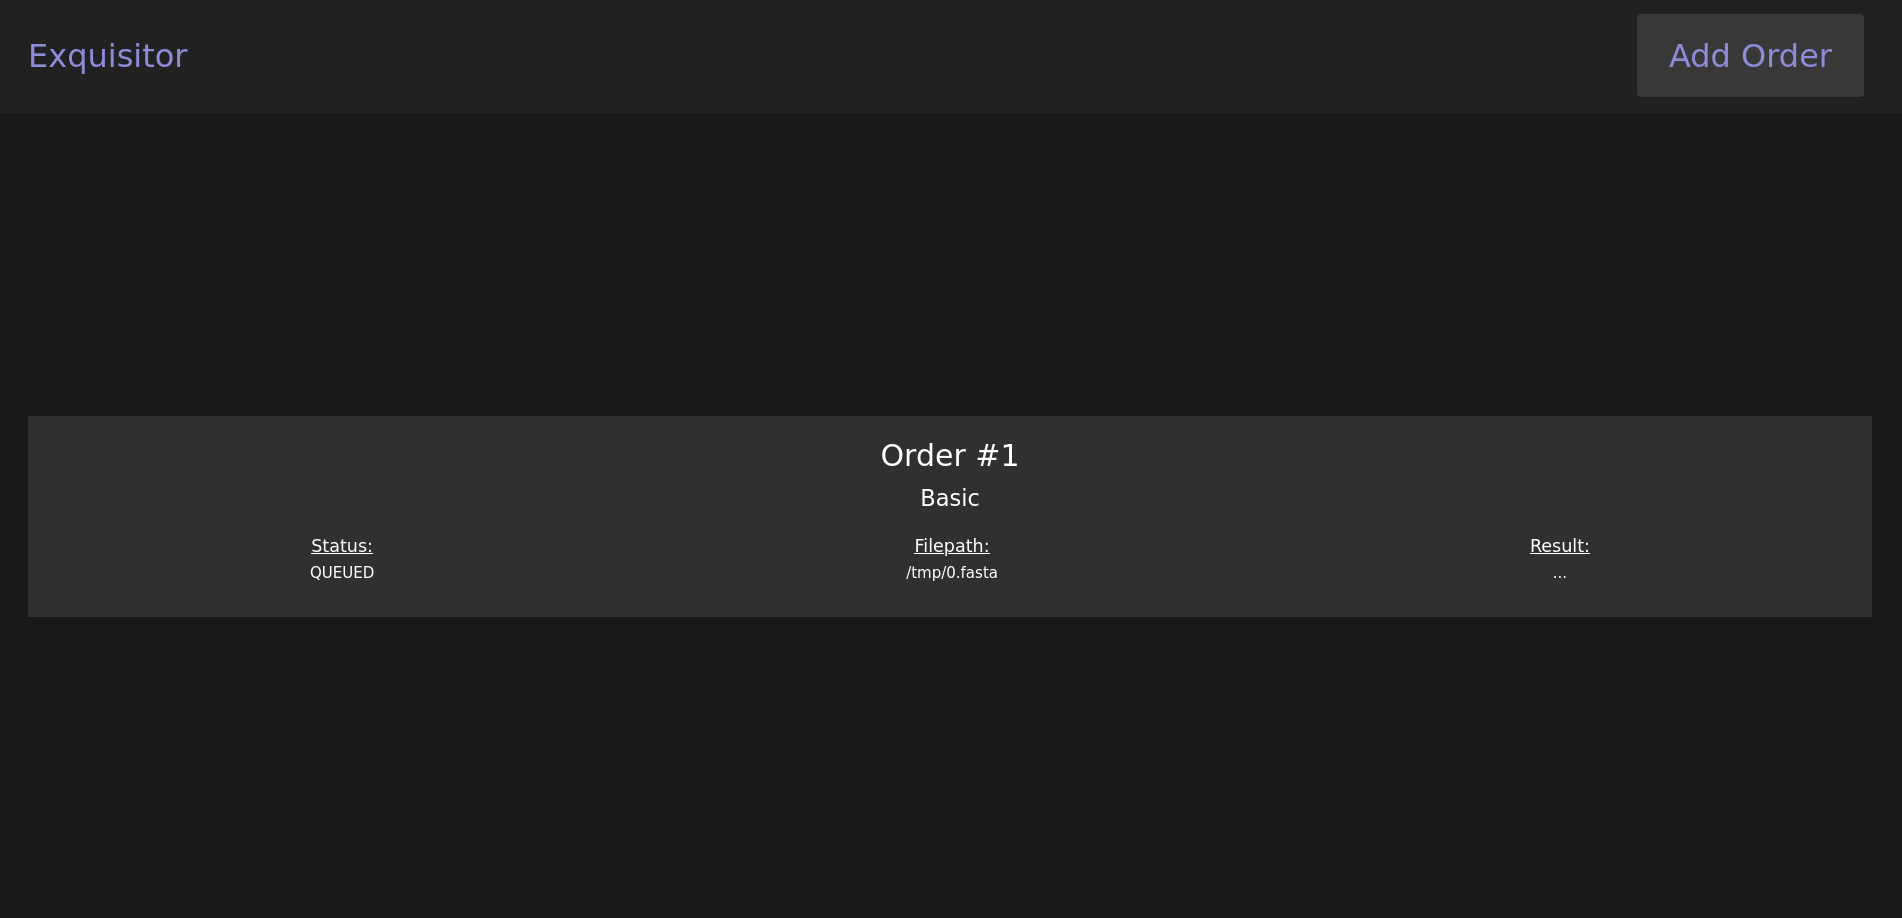
\includegraphics[width=\textwidth]{tex/pictures/app/web_search_success.png}
                    \end{center}
                    \caption{
                        Strona zlecenia.
                    }\label{Picture:App:WebSearchSuccess}
                \end{figure}

                \begin{figure}
                    \begin{center}
                        
\includegraphics[width=\textwidth]{tex/pictures/app/web_search_failure.png}
                    \end{center}
                    \caption{
                        Strona z komunikatem o błędzie wyszukiwania zlecenia.
                    }\label{Picture:App:WebSearchFailure}
                \end{figure}

                \begin{longtblr}[
                    caption = {Składnia poleceń aplikacji konsolowej.},
                    label = {Table:ConsoleCommandsSyntax}
                ]{
                    colspec = {| >{\footnotesize}m{0.2\textwidth} | >{\footnotesize}m{0.2\textwidth} | >{\footnotesize}X |},
                    rowhead = 1,
                }
                    \hline
                    \textbf{\normalsize Polecenie}     & \textbf{\normalsize Argument}    & \textbf{\normalsize Opis argumentu} \\*
                    \hline \hline

                    \multirow{4}{*}{\texttt{experiment}}  & \texttt{-\phantom{}-resolution <liczba>}   & Rozdzielczość monitorowania eksperymentu w sekundach. Określa jak często będzie sprawdzane wykorzystanie zasobów przez eksperyment, oraz przekroczenie czasu trwania eksperymentu. \\*
                                                          & \texttt{-\phantom{}-command <polecenie>}   & Polecenie, które zostanie wykonane jako eksperyment. Powinno to być poprawne polecenie aplikacji konsolowej. \\*
                                                          & \texttt{-\phantom{}-output <ścieżka>}      & Ścieżka do pliku, w którym zostaną zapisane wyniki monitorowania eksperumentu. Wyniki zapisywane są jako tabela w formacie CSV. \\*
                                                          & \texttt{-\phantom{}-max-duration <liczba>} & Maksymalny czas trwania eksperymentu w sekundach. Po przekroczeniu czasu trwania eksperymentu nastąpi jego przerwanie. \\ \hline

                    % % compare             & \texttt{
                            
                    % % } \\ \hline % @TODO

                    \multirow{3}{*}{\texttt{compare-clusters}}  & \texttt{-\phantom{}-reference <ścieżka>} & Ścieżka do pliku z wynikami klasyfikacji taksonomicznej, które stanowią punkt odniesienia w porównaniu. \\*
                                                                & \texttt{-\phantom{}-second <ścieżka>}    & Ścieżka do pliku z wynikami klasyfikacji taksonomicznej, które zostaną porównane względem wskazanych wyników referencyjnych. \\*
                                                                & \texttt{[-\phantom{}-output <ścieżka>]}  & Ścieżka do pliku, w którym zostaną zapisane wyniki dokonanego porównania. \\ \hline

                    \multirow{4}{*}{\texttt{search}}    & \texttt{-\phantom{}-input <ścieżka>}    & Ścieżka do pliku, który zawiera sekwencje DNA. \\*
                                                        & \texttt{-\phantom{}-output <ścieżka>}   & Ścieżka do pliku, w którym zostaną zapisane wyniki wyszukiwania. \\*
                                                        & \texttt{-\phantom{}-blast <ścieżka>}    & Ścieżka do pliku wykonywalnego \texttt{blastn}. \\*
                                                        & \texttt{-\phantom{}-blast-db <ścieżka>} & Ścieżka do folderu z bazą danych nukleotydów \texttt{nt}. \\ \hline

                    \multirow{13}{*}{\texttt{run}}      & \texttt{-\phantom{}-input <ścieżka>}           & Ścieżka do pliku, który zawiera sekwencje DNA. \\*
                                                        & \texttt{-\phantom{}-output <ścieżka>}          & Ścieżka do pliku, w którym zostaną zapisane wyniki klasyfikacji taksonomicznej. \\*
                                                        & \texttt{-\phantom{}-file-format <file-format>} & Format pliku z sekwencjami DNA. Dostępne formaty: \texttt{fasta}, \texttt{fastq} oraz \texttt{auto} (automatyczne wykrywanie formatu na podstawie rozszerzenia pliku). \\*
                                                        & \texttt{-\phantom{}-pipeline <pipeline>}       & Metoda wykorzystana do określania niepodobieństwa między sekwencjami DNA. Dostępne metody: \texttt{basic} (zmodyfikowany algorytm Needlemana-Wunscha), \texttt{k-mer} (zanurzenia k-merów), \texttt{neural} (sieć neuronowa). \\*
                                                        & \texttt{-\phantom{}-cluster <cluster>}         & Algorytm grupowania. Dostępne algorytmy: \texttt{k-medoid}. \\*
                                                        & \texttt{-\phantom{}-k <liczba>}                & Liczba grup tworzonych przez algorytm grupowania. \\*
                                                        & \texttt{-\phantom{}-blast <ścieżka>}           & Ścieżka do pliku wykonywalnego \texttt{blastn}. \\*
                                                        & \texttt{-\phantom{}-blast-db <ścieżka>}        & Ścieżka do folderu z bazą danych nukleotydów \texttt{nt}. \\*
                                                        & \texttt{[-\phantom{}-gap-penalty <liczba>]}    & Parametr kary za przerwę w metodzie z wykorzystaniem zmodyfikowanego algorytmu Needlemana-Wunscha. Argument obowiązkowy przy podaniu \texttt{basic} jako wartości argumentu \texttt{-{}-pipeline}. \\*
                                                        & \texttt{[-\phantom{}-kmer <ścieżka>]}          & Długość wykorzystanych k-merów w metodzie zanurzeń k-merów. Argument obowiązkowy przy podaniu \texttt{k-mer} jako wartości argumentu \texttt{-{}-pipeline}. \\*
                                                        & \texttt{[-\phantom{}-model <ścieżka>]}         & Ścieżka do pliku, który zawiera zapisane wagi modelu sieci neuronowej. Argument obowiązkowy przy podaniu \texttt{neural} jako wartości argumentu \texttt{-{}-pipeline} .\\*
                                                        & \texttt{[-\phantom{}-only-cluster]}            & Flaga, której użycie powoduje przerwanie potoku przetwarzania po przeprowadzeniu grupowania sekwencji.  \\*
                                                        & \texttt{[-\phantom{}-save-clusters}            & Flaga, której użycie powoduje zapisanie wyników grupowania do pliku. \\ \hline
                \end{longtblr}

    % ===== ===== ===== =====
    % OPIS TESTÓW JEDNOSTKOWYCH
    % ===== ===== ===== =====
    \subsection{Testy}

        \subsubsection{Testy jednostkowe}

            Testy jednostkowe zostały przeprowadzone w celu weryfikacji poprawności działania poszczególnych funkcji i metod w izolacji. Testy obejmowały zarówno typowe scenariusze wykorzystania funkcjonalności, jak i potencjalne sytuacje błędne.
            
            \paragraph{Zakres}  
            Testy jednostkowe objęły większość funkcji oraz metod w bibliotece \texttt{exquisitor-core}. Szczególną uwagę poświęcono poprawności działania funkcji związanych z wczytywaniem sekwencji oraz obliczaniem miar.
            
            \paragraph{Narzędzia}  
            Wykorzystano wbudowane narzędzie \texttt{cargo test} języka Rust, do uruchamiania testów jednostkowych. Narzędzie to automatycznie uruchamia testy zawarte w plikach implementacyjnych, traktując je jako testy jednostkowe.

            \paragraph{Pokrycie testami}
            Do sprawdzenia stopnia pokrycia kodu testami wykorzystano narzędzie \texttt{tarpaulin}\cite{Rust:tarpaulin}. 
            Osiągnięto \textbf{65\%} pokrycia linii kodu za pomocą testów jednostkowych.

        \subsubsection{Testy manualne}
        
            \paragraph{Zakres}
            Testy manualne objęły działanie interfejsu użytkownika aplikacji konsolowej oraz aplikacji internetowej W przypadku aplikacji konsolowej sprawdzono działanie wszystkich poleceń z uwzględnieniem klasycznych sytuacji błędnych. W aplikacji intenretowej testowano funkcjonalności: dodawania, wyszukiwania i przeglądania zleceń.

            \paragraph{Metoda}
            Ręczne wykonywanie scenariuszy testowych, takich jak:
            \begin{itemize}
                \item {Dodanie nowego zlecenia i weryfikacja czy wyświetla się na stronie głównej aplikacji internetowej.}
                \item {Wyszukanie dodanego zlecenia po identyfikatorze na stronie głównej.}
                \item {Uruchomienie polecenia aplikacji konsolowej wyszukiwania w bazie danych i sprawdzenie, czy powstał odpowiedni plik z wynikami.}
            \end{itemize}
